\documentclass[10pt]{beamer}

\usetheme{McMaster}
\usepackage{math}

%===Specific for this talk===%
\usepackage{algorithm,algorithmicx,algpseudocode}
\DeclareMathOperator{\iaa}{IAA} % paper specific
\newtheorem{proposition}{Proposition}
\newcommand{\vecw}{\left ( \vec{w}_i^n \right )^\top}
\newcommand{\Aij}{\left ( \hat{A} + E_{i \to j}^{n} \right )^{-1}}
\newcommand{\AijE}{\Aij E_{i \to j}^{n}}
\DeclareMathOperator{\Span}{span}
\DeclareMathOperator{\argmin}{argmin}
\usepackage{tikz, pgfplots}
\usepackage{tikz-3dplot}
\usetikzlibrary{decorations.pathreplacing,positioning,calc,intersections,3d,shapes.geometric,shapes,chains,math,fit,backgrounds}

\tikzset{
	pics/starred/.style={code={
		\filldraw[magenta] (0,0) -- (0,1) -- (1,1) -- (1,0) -- cycle;
		\filldraw[black, opacity=0.2] (0,1) -- (1,0) -- (0,0) -- cycle;
		\filldraw[black, opacity=0.4] (0,0) -- (1,1) -- (0,1) -- cycle;
%		\filldraw[red] (0,0) -- (0.5,0.5) -- (0,1) -- cycle;
%		\filldraw[blue] (0,1) -- (0.5,0.5) -- (1,1) -- cycle;
%		\filldraw[green] (1,1) -- (0.5,0.5) -- (1,0) -- cycle;
%		\filldraw[yellow] (1,0) -- (0.5,0.5) -- (0,0) -- cycle;
%		\filldraw[black, opacity=0.3] (1,0) -- (1,1) -- (0.5,1) -- (0.5,0) -- cycle;
%		\node[star, fill=magenta!30!black] at (0.5,0.5) {};
	}}
}

%===School colours===%
\definecolor{MacMaroon}{HTML}{7A003C} % Primary (dark)
\definecolor{UnigePink}{RGB}{207,0,99}
\definecolor{UnigeGreen}{RGB}{0,126,100}
\definecolor{SFURed}{HTML}{CC0633}
\definecolor{SFUDarkRed}{HTML}{A6192E}
\definecolor{uLavalGold}{RGB}{255,193,3}
\definecolor{uLavalRed}{RGB}{227,5,19}

\title{Globalization techniques for MSPIN on phase-field fracture models}
\author{Conor McCoid}
\institute{Joint work with Blaise Bourdin at McMaster University}
\date{May 21st, 2025}

\renewcommand*{\thefootnote}{\fnsymbol{footnote}}

\begin{document}

\maketitle

\begin{frame}{Outline}

\begin{enumerate}
\item Introduction to domain decomposition and Schwarz methods
\item Newton-Schwarz methods
	\begin{enumerate}
	\item Phasefield fracture model and AltMin
	\item MSPIN and parallelogram minimization
	\end{enumerate}
\end{enumerate}
\end{frame}

\section{Introduction to domain decomposition and Schwarz methods} % 15 min

% Schwarz (incl. keyhole domain)
\begin{frame}{H.A. Schwarz, 1869}

How do we solve the Laplace equation ($\Delta u =0$) on complicated domains?

We split the domain into simpler subdomains.

\begin{figure}
	\centering
	\begin{tikzpicture}
		\begin{scope}[blend group = soft light]
			\filldraw[draw=black, fill=red!50!white, thick] (0,0) circle (1.5);
			\filldraw[draw=black, fill=green!50!white, thick] (0,-1) rectangle (3,1);
		\end{scope}
		\node[left] at (-1.5,0) {$\Omega_1$};
		\node[right] at (3,0) {$\Omega_2$};
		\node[left] at (0,0) {$\Gamma_2$};
		\node[right] at (1.5,0) {$\Gamma_1$};
	\end{tikzpicture}
%\vspace{-3em}
%
\includegraphics[width=0.5\textwidth]{AOSM/FIG_keyhole.png}
%\vspace{-4em}
%\caption{Schwarz's original example, taken from wikimedia.org}
\end{figure}

Alternating Schwarz method:
\begin{equation*}
	\begin{cases} \Delta u_1^{n+1} = 0 & \text{in } \Omega_1, \\ u_1^{n+1} = u_2^n & \text{on } \Gamma_1, \end{cases}
	\quad
	\begin{cases} \Delta u_2^{n+1} = 0 & \text{in } \Omega_2, \\ u_2^{n+1} = u_1^{n+1} & \text{on } \Gamma_2. \end{cases}
\end{equation*}
\end{frame}

\begin{frame}{Simple example}

\begin{equation*}
	u''(x) = -1, \quad x \in [-1,1], \quad u(-1)=u(1) = 0
\end{equation*}
\begin{equation*}
	\Omega_1 = [-1,0.18], \quad \Omega_2 = [-0.22, 1]
\end{equation*}

\begin{figure}
	\only<1>{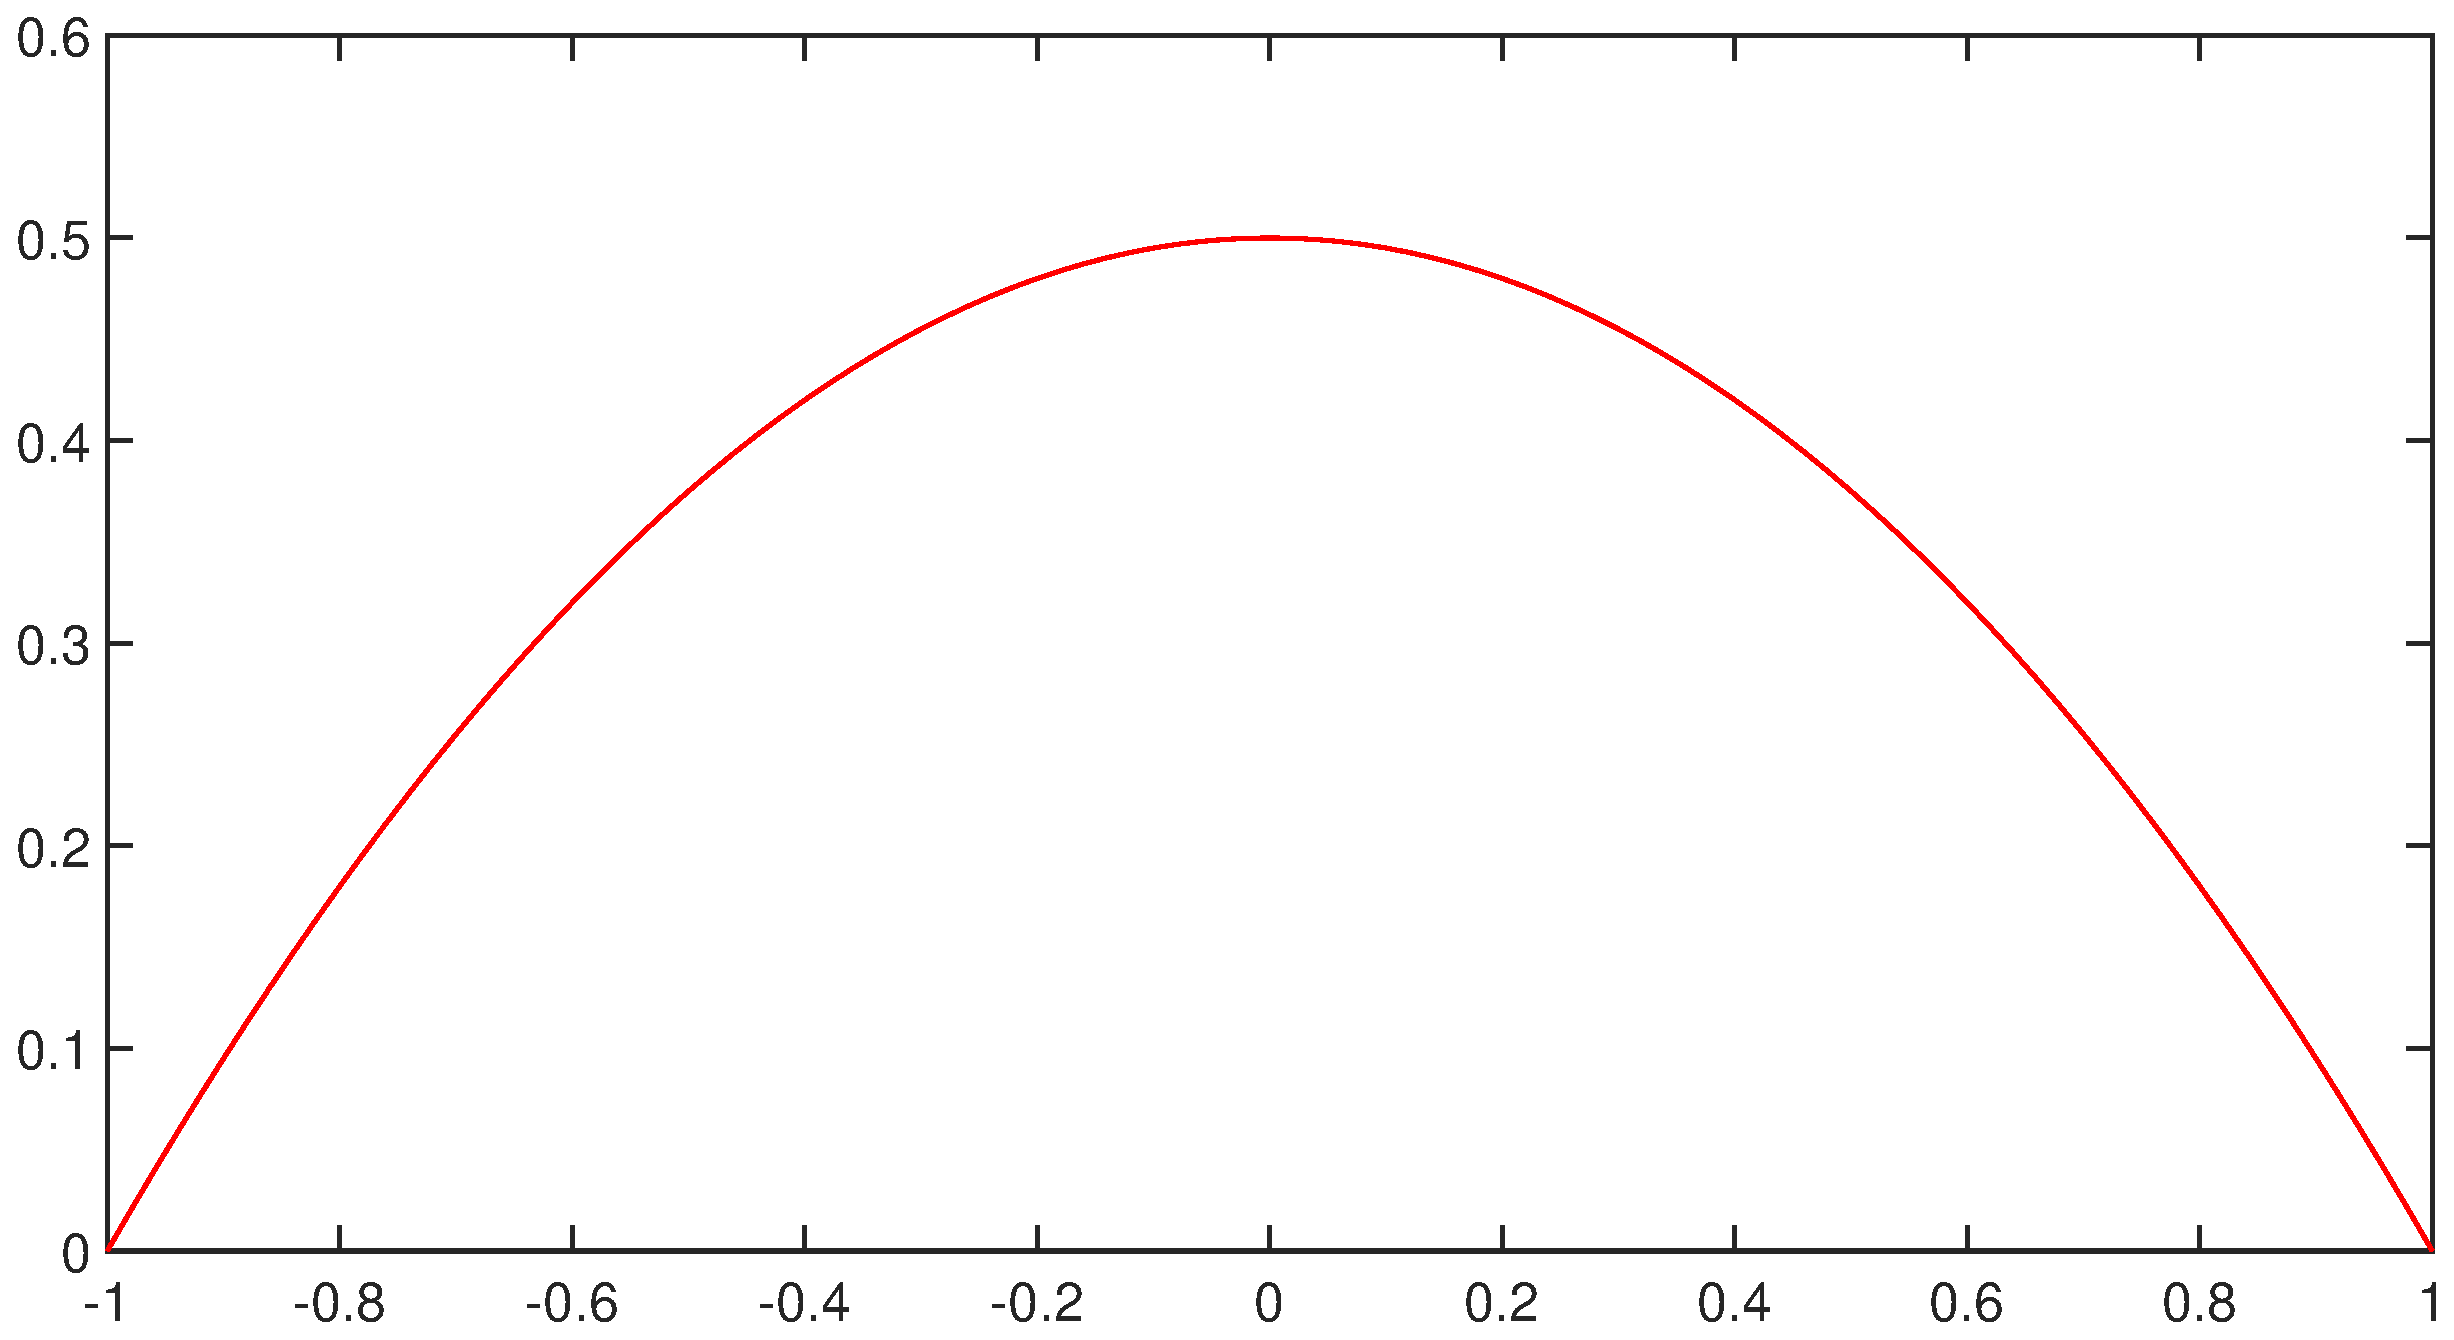
\includegraphics[width=\textwidth]{../AOSM/PLOT_SimpleSchwarz1.eps}}
	\only<2>{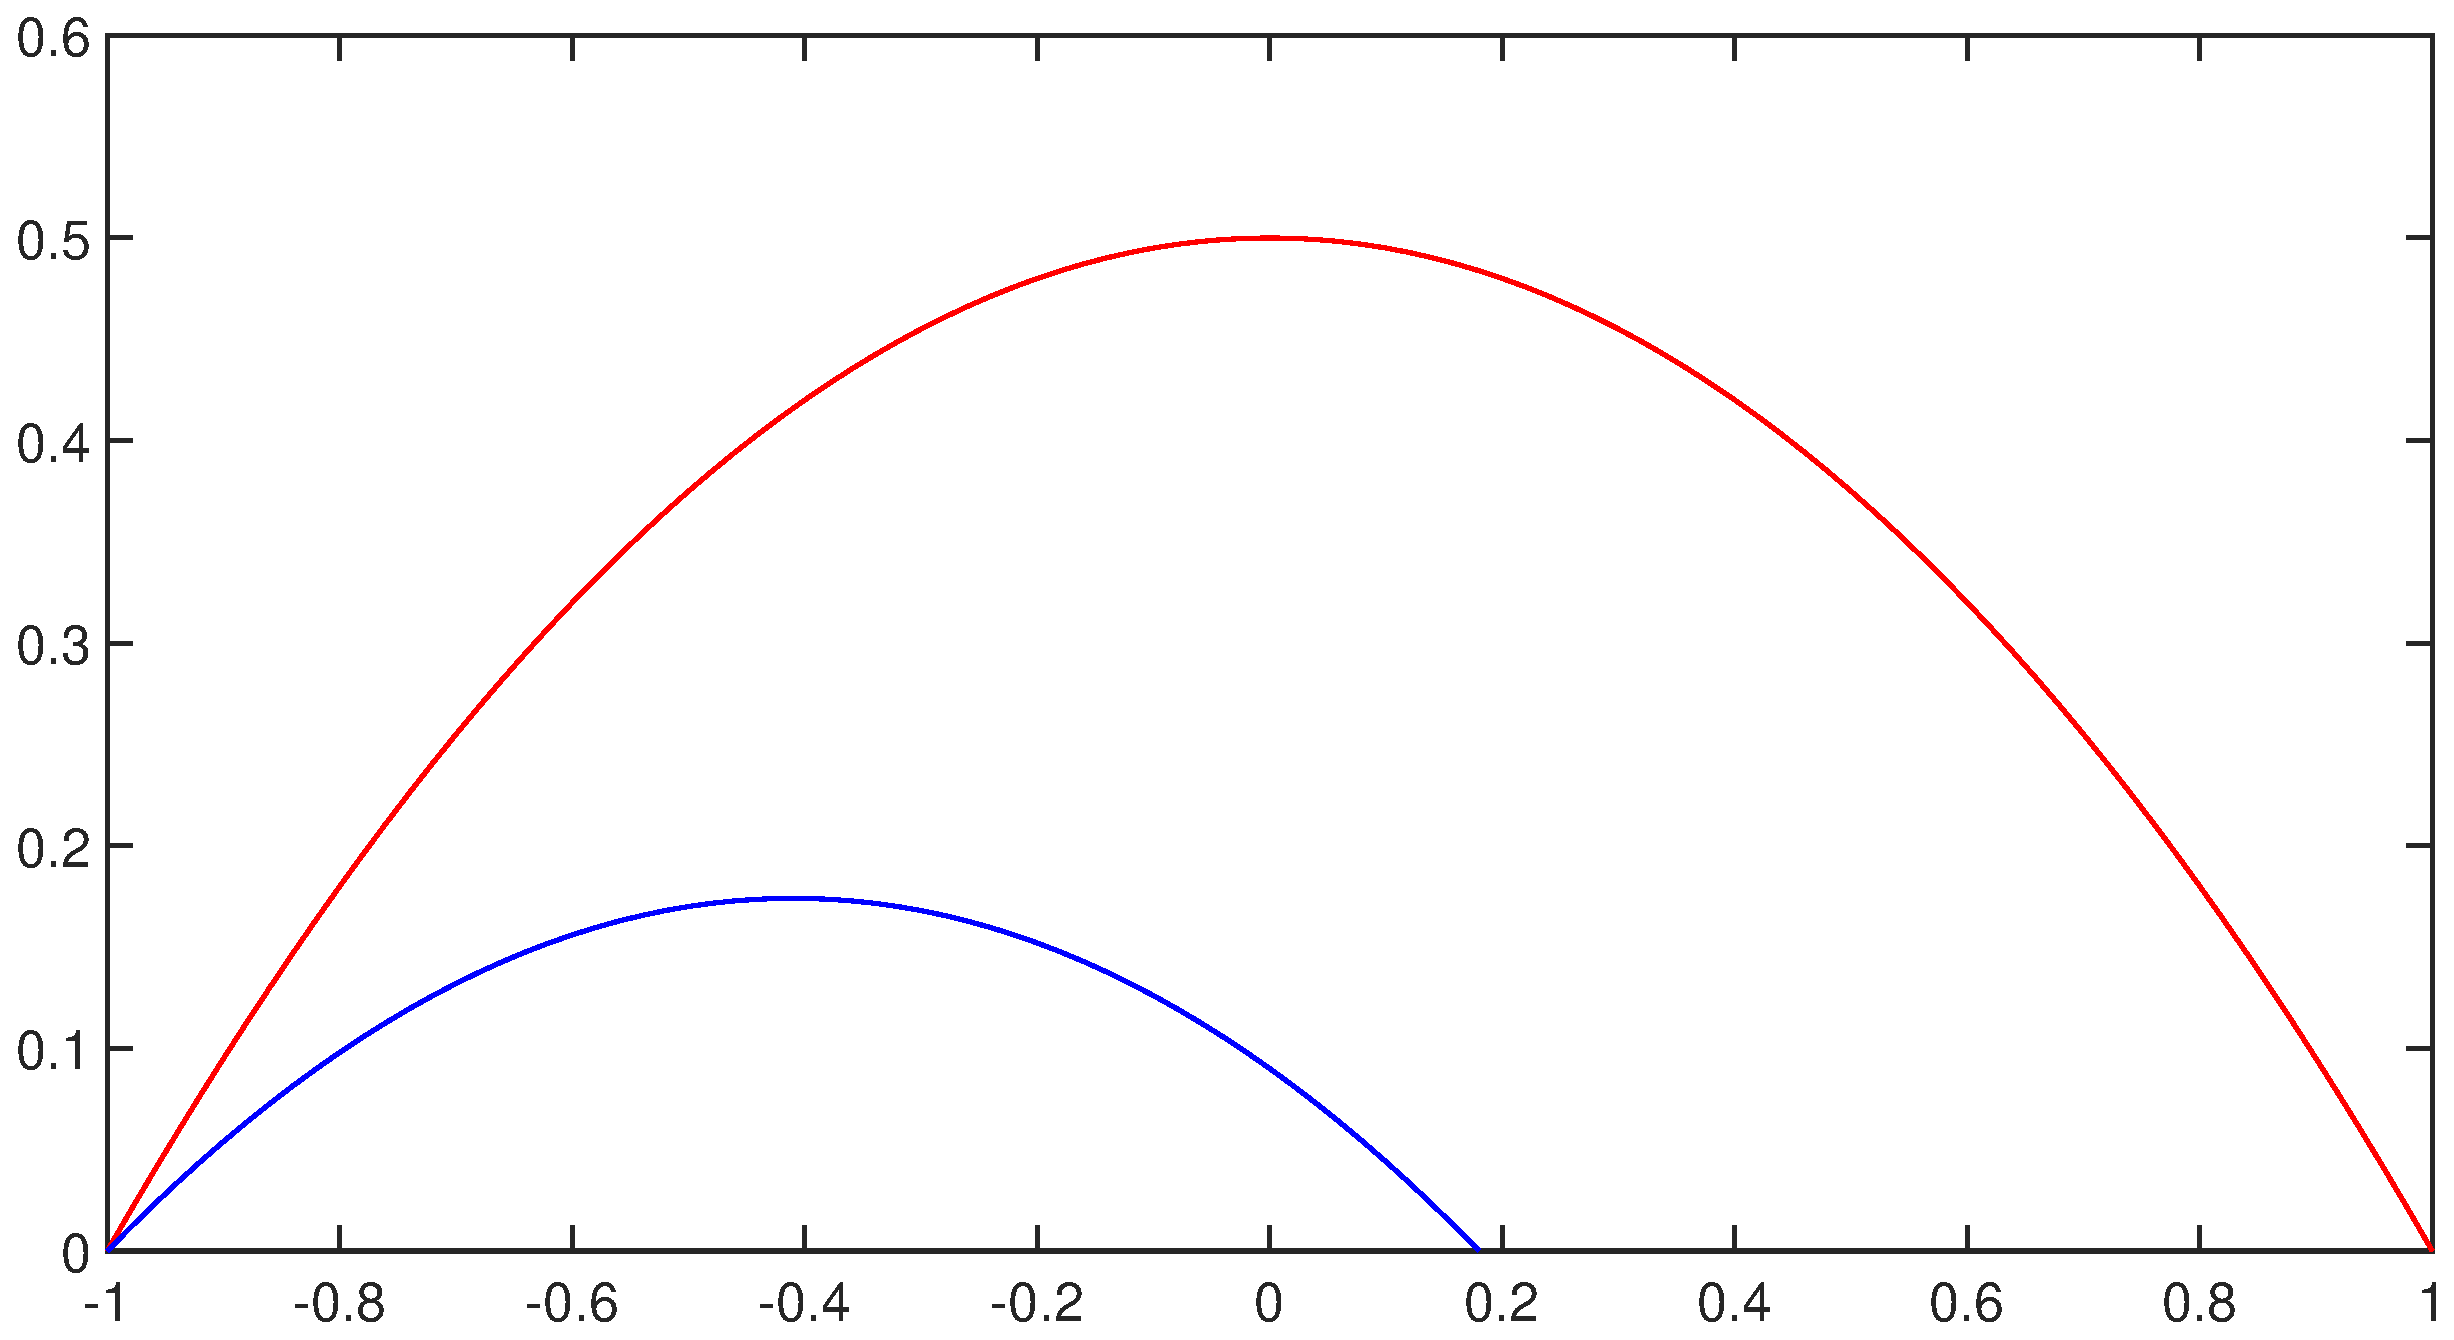
\includegraphics[width=\textwidth]{../AOSM/PLOT_SimpleSchwarz2.eps}}
	\only<3>{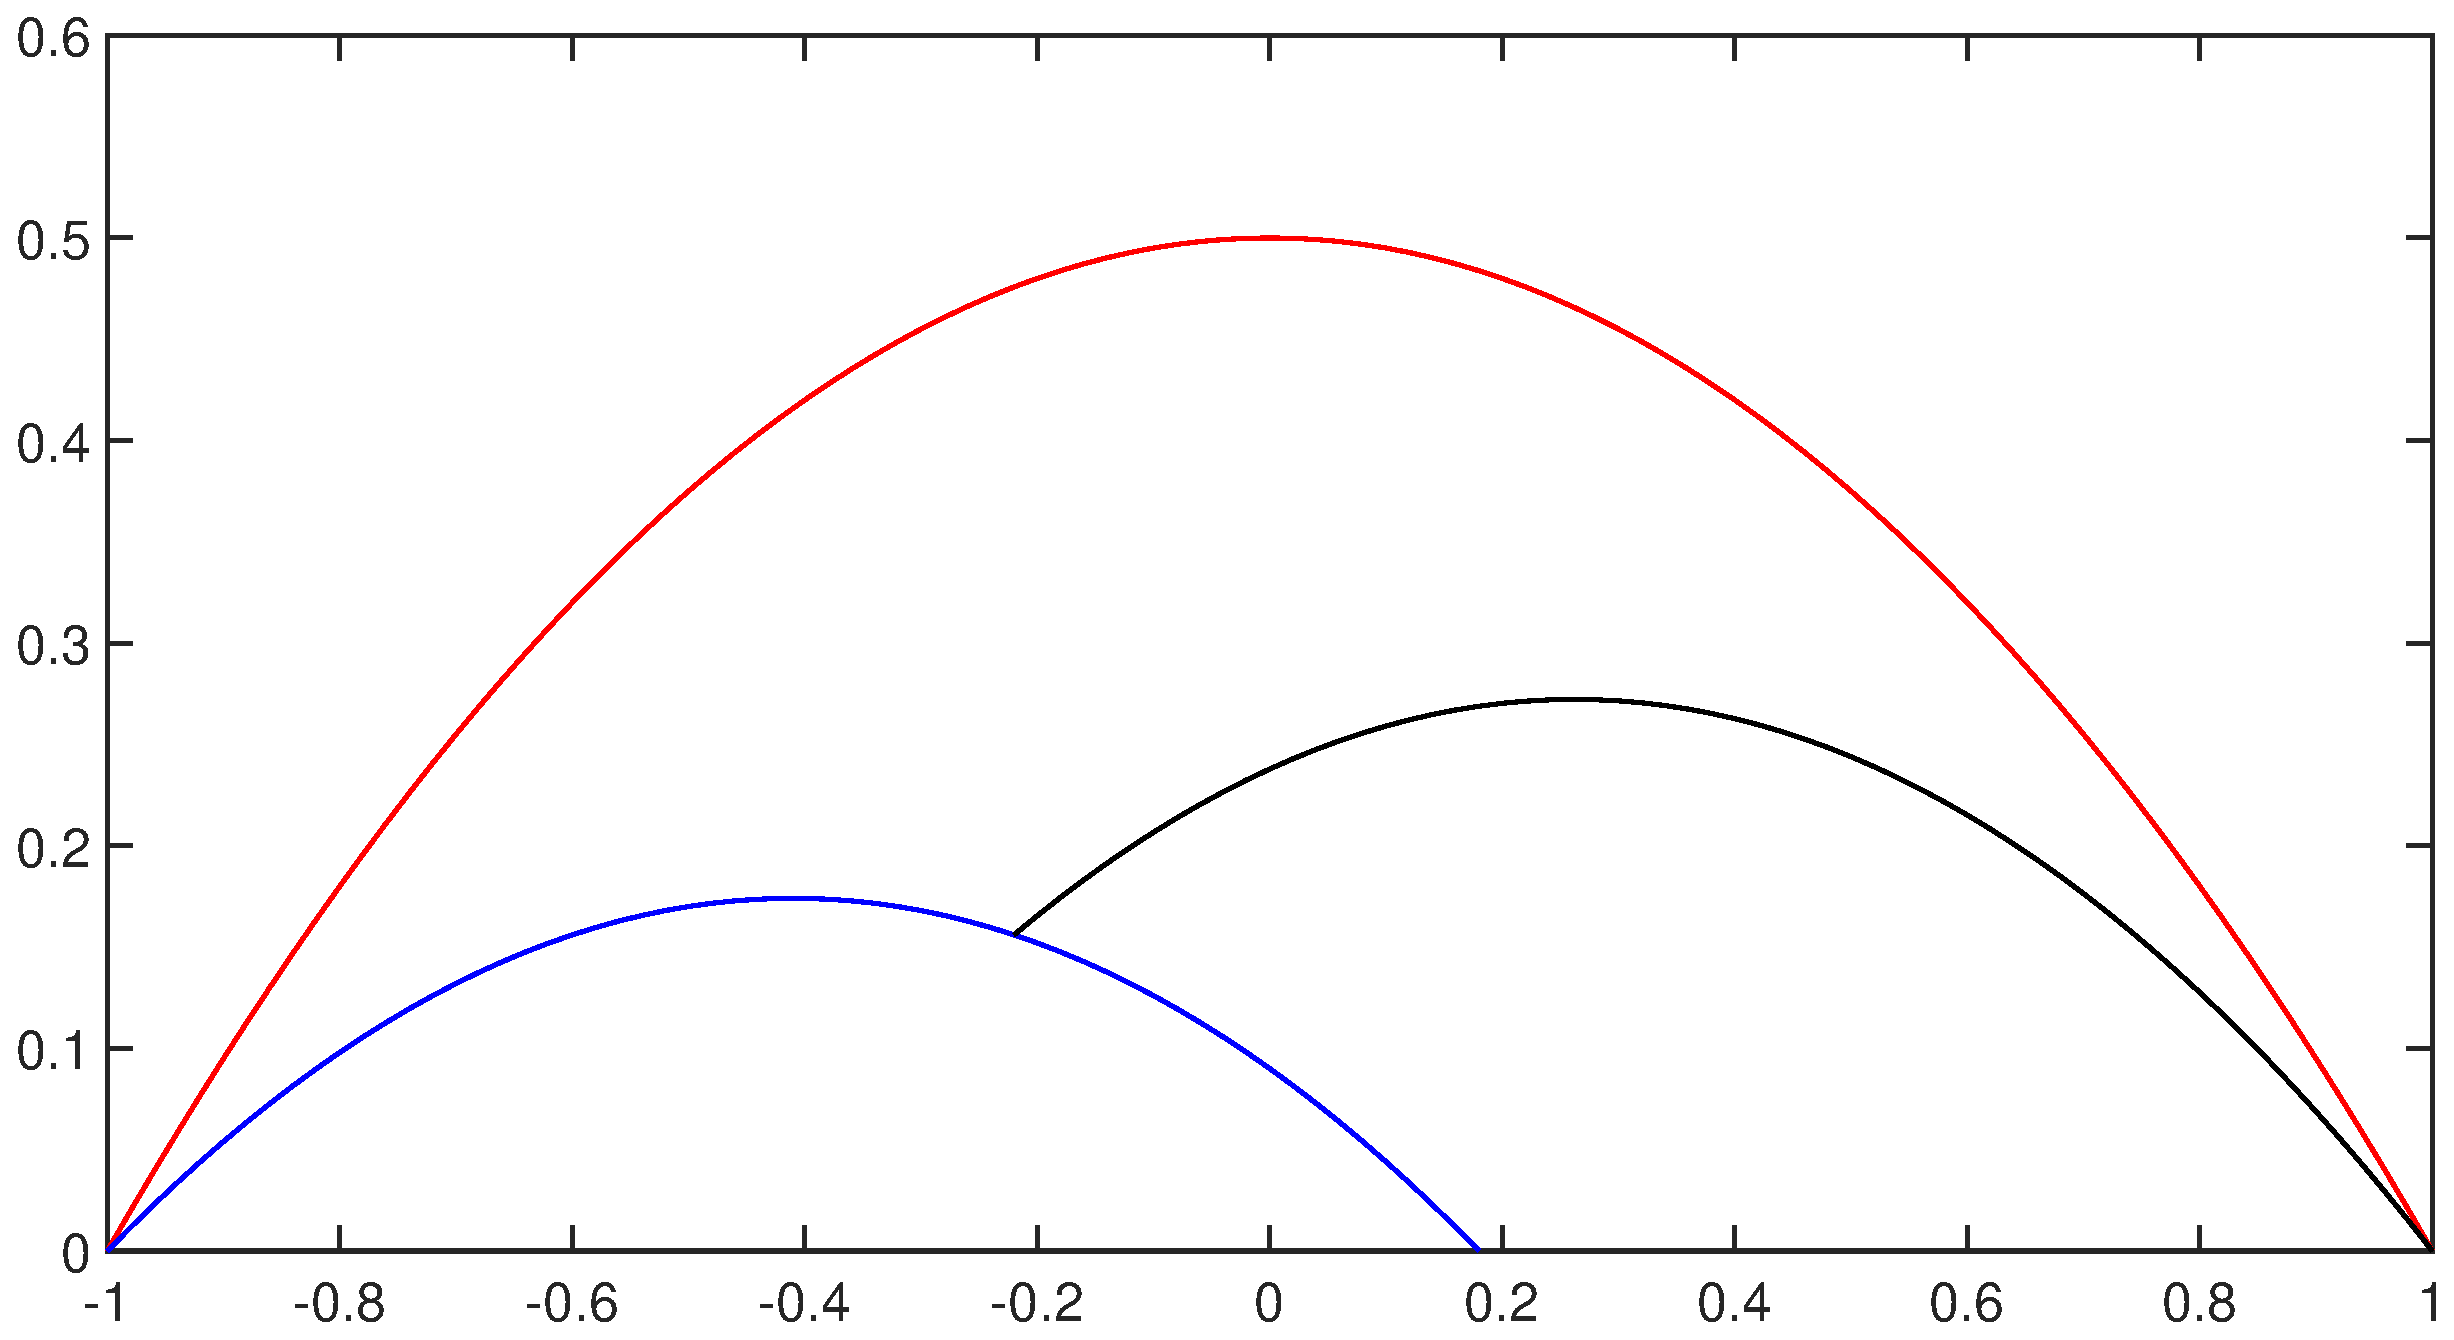
\includegraphics[width=\textwidth]{../AOSM/PLOT_SimpleSchwarz3.eps}}
	\only<4>{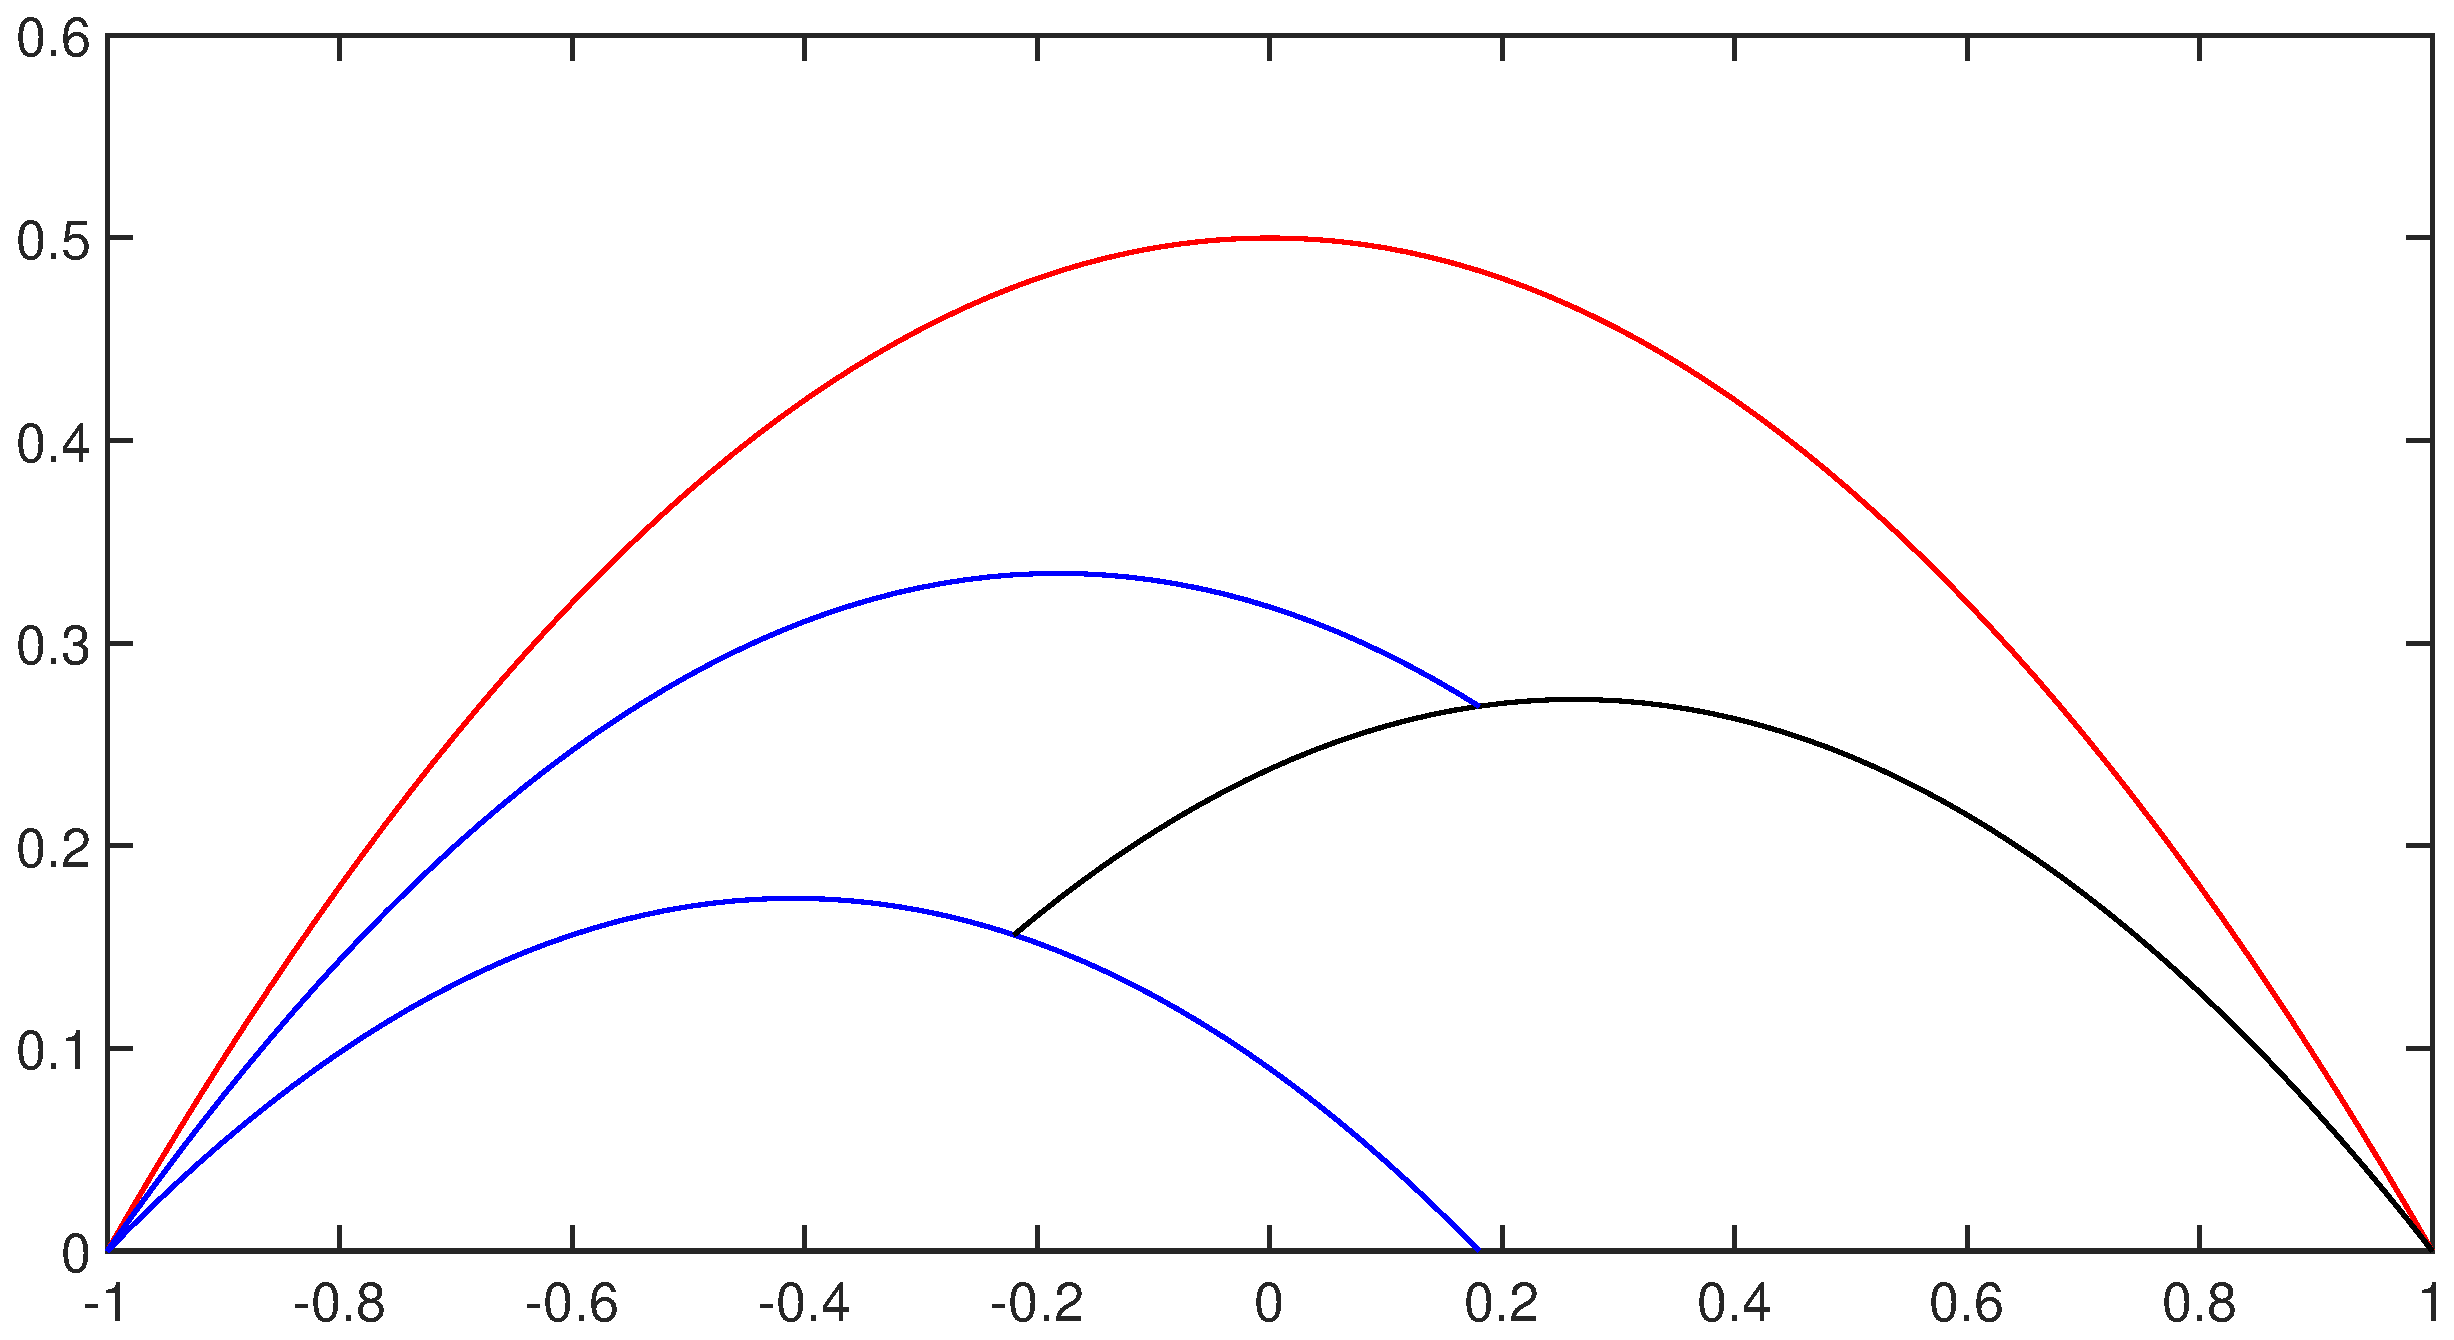
\includegraphics[width=\textwidth]{../AOSM/PLOT_SimpleSchwarz4.eps}}
	\only<5>{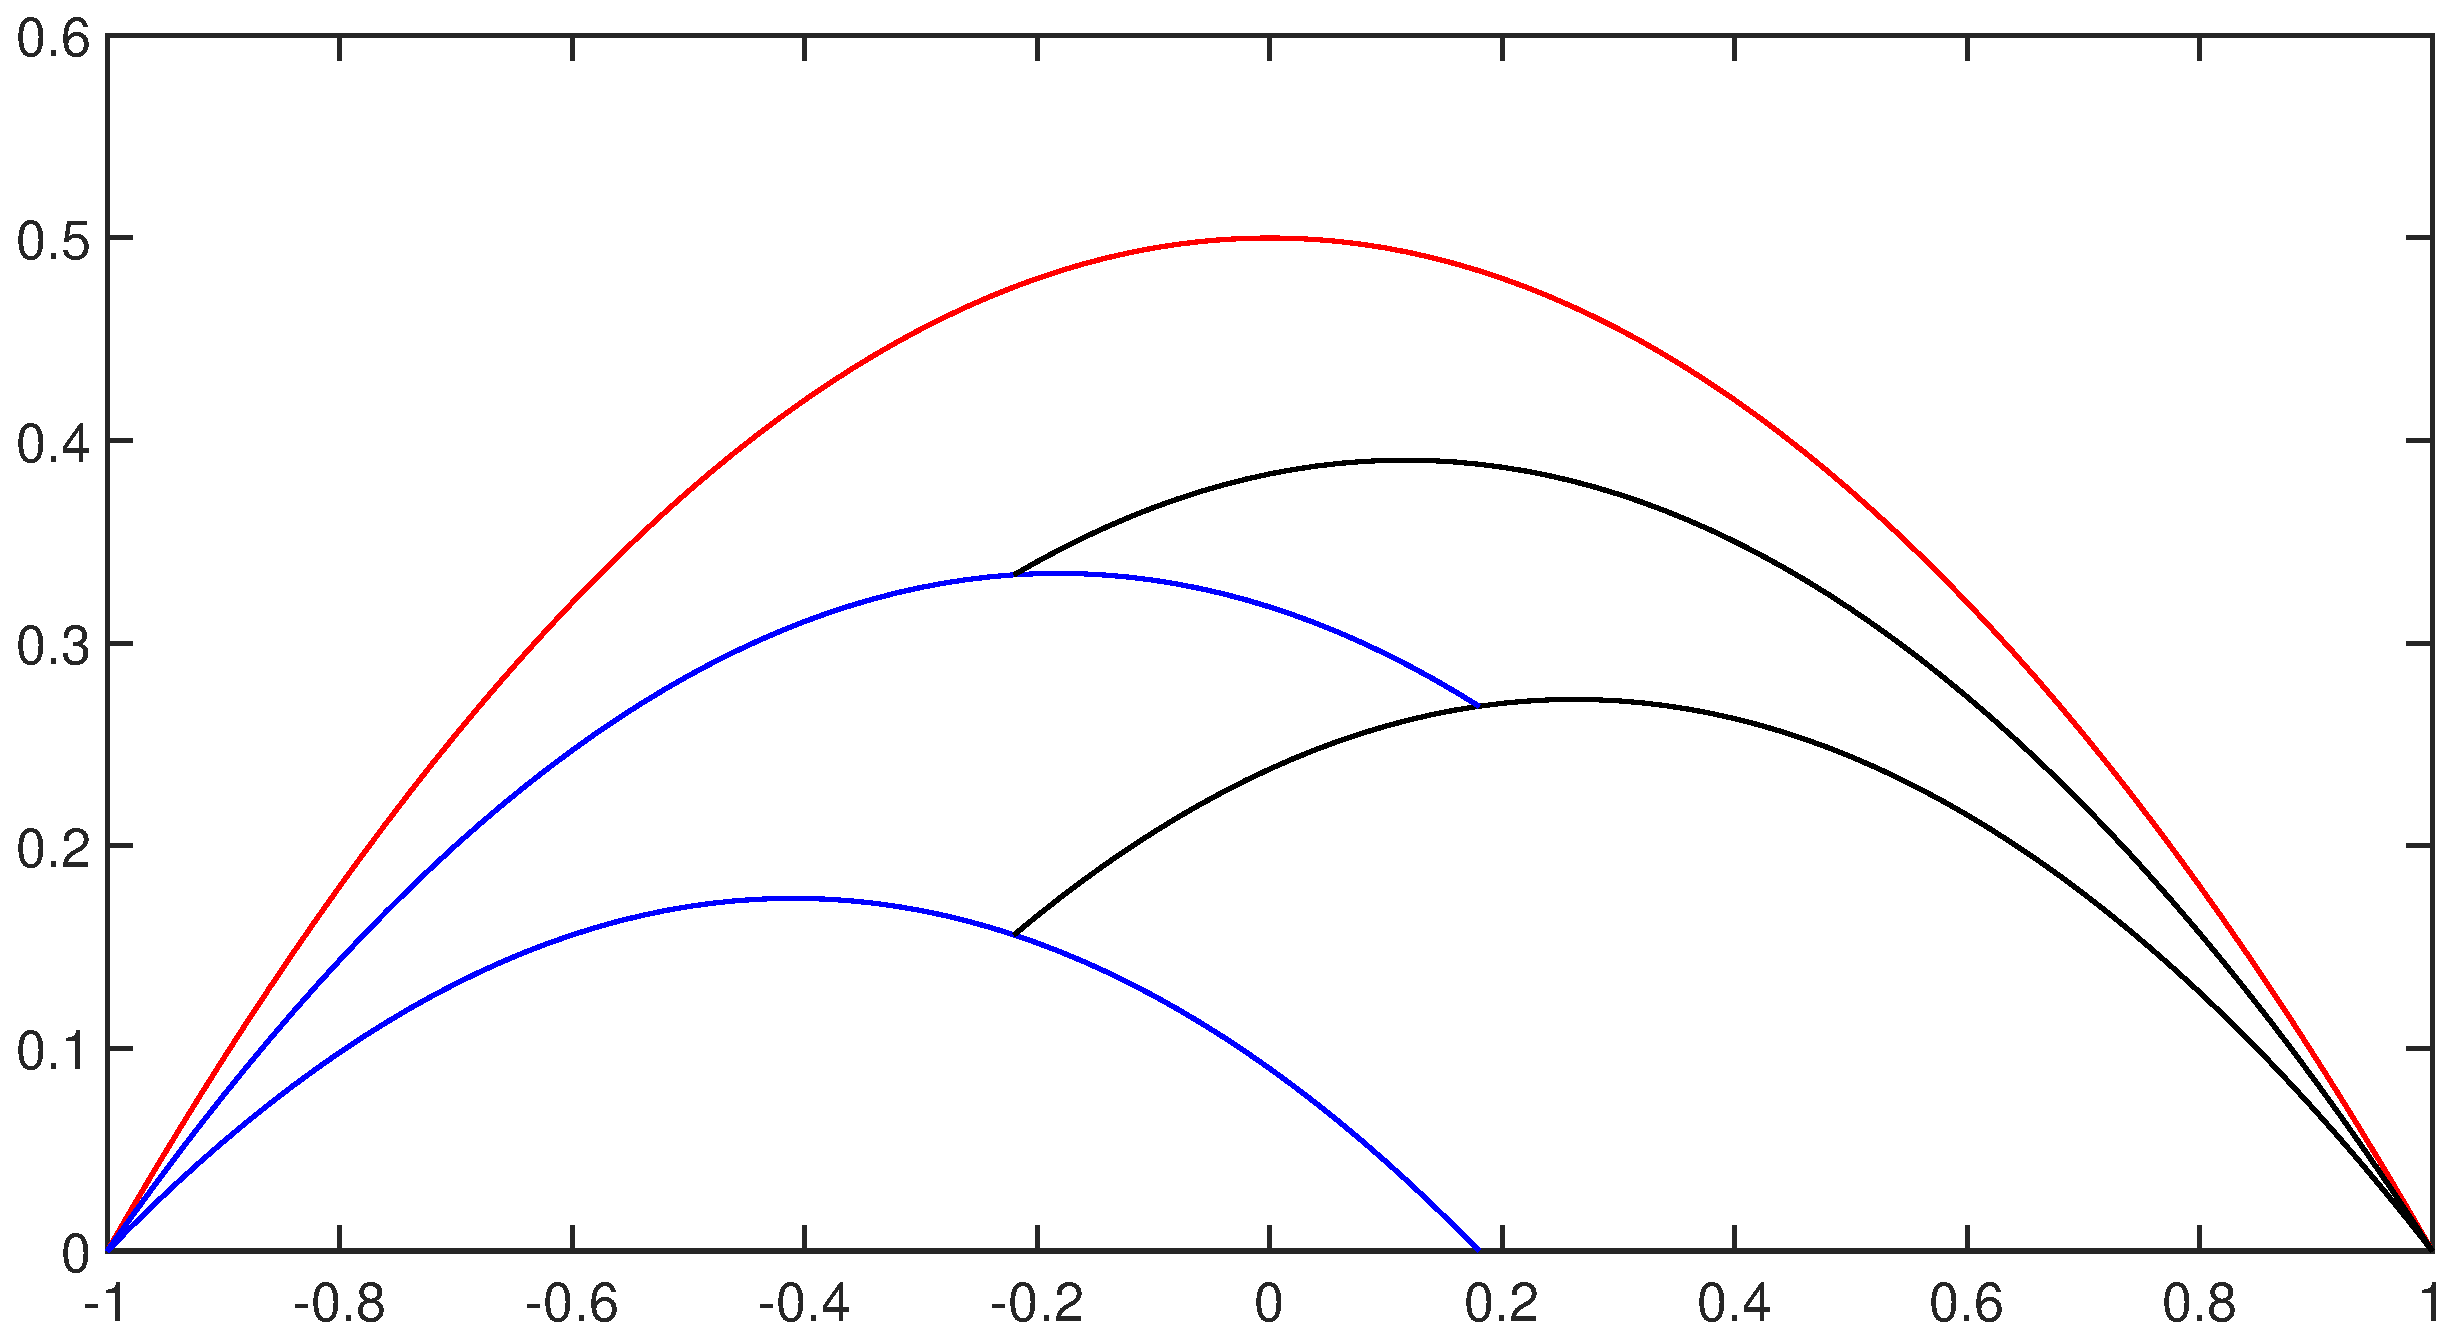
\includegraphics[width=\textwidth]{../AOSM/PLOT_SimpleSchwarz5.eps}}
\end{figure}
\end{frame}

\begin{frame}
\frametitle{Field-split Schwarz methods}

Instead of splitting up the physical domain, we can split up the problem into fields.

Suppose a problem can be written as
\begin{equation*}
	\begin{bmatrix} F(u,v) \\ G(u,v) \end{bmatrix} = \begin{bmatrix} f \\ g \end{bmatrix},
\end{equation*}
where $F$ depends more strongly on $u$ and $G$ depends more strongly on $v$.

Field-split multiplicative Schwarz:
\begin{equation*}
	F(u^{(n+1)},v^{(n)}) = f, \quad G(u^{(n+1)},v^{(n+1)}) = g.
\end{equation*}

%A simple example:
%\begin{equation*}
%	\begin{bmatrix} v \exp(u) \\ u \exp(v) \end{bmatrix} = \begin{bmatrix} f \\ g \end{bmatrix}
%\end{equation*}

\end{frame}

%% ASPIN/MSPIN/RASPEN
%\begin{frame}{Schwarz as a fixed point iteration}
%
%Schwarz methods can be represented as fixed point iterations:
%\begin{equation*}
%	u^{n+1} = g \left ( u^{n-1} \right ),
%\end{equation*}
%where $g(u)$ represents one iteration of a Schwarz method that takes boundary data from the input $u$.
%
%The fixed point of $g$ is the solution on the first subdomain.
%This is also the root of the function $f(u) = g(u) - u$.
%We apply Newton's method:
%\begin{equation*}
%	u^* = u^{n-1} - J(u^{n-1})^{-1} f(u^{n-1}),
%\end{equation*}
%where $J$ is the Jacobian of the function $f$.
%\end{frame}
%
%\begin{frame}{Schwarz-Preconditioned Newton methods (Cai \& Keyes, 2001)}
%
%This is equivalent to preconditioning Newton's method with a Schwarz method.
%
%Let
%\begin{equation*}
%	f(u) = \begin{bmatrix} f_1(u_1, u_2) \\ f_2(u_1,u_2) \end{bmatrix}.
%\end{equation*}
%Then Newton's method tells us to solve the nonlinear problem
%\begin{equation*}
%	\begin{bmatrix} J_{11}^{(n+1)} & J_{12}^{(n+1)} \\ J_{21}^{(n+1)} & J_{22}^{(n+1)} \end{bmatrix} \begin{bmatrix} u_1^{n+1} - u_1^n \\ u_2^{n+1} - u_2^n \end{bmatrix} = \begin{bmatrix} f_1 \\ f_2 \end{bmatrix},
%\end{equation*}
%where $J_{ij}^{(n+1)}$ is the derivative of $f_i$ with respect to $u_j$ evaluated at $u_1^{n+1}$ and $u_2^{n+1}$.
%\end{frame}
%
%\begin{frame}{Schwarz-Preconditioned Newton methods (Cai \& Keyes, 2001)}
%
%Preconditioning this with a parallel Schwarz method tells us to solve
%\begin{equation*}
%	\begin{bmatrix} J_{11}^{(n+1)} \\ & J_{22}^{(n+1)} \end{bmatrix} \begin{bmatrix} u_1^{n+1} - u_1^n \\ u_2^{n+1} - u_2^n \end{bmatrix} = \begin{bmatrix} f_1 \\ f_2 \end{bmatrix} - \begin{bmatrix} & J_{12}^{(n)} \\ J_{21}^{(n)} \end{bmatrix} \begin{bmatrix} u_1^{n} - u_1^{n-1} \\ u_2^{n} - u_2^{n-1} \end{bmatrix},
%\end{equation*}
%and completing the iteration by solving
%\begin{equation*}
%	\begin{bmatrix} J_{11}^{(n+1)} \\ & J_{22}^{(n+1)} \end{bmatrix}^{-1} \begin{bmatrix} J_{11}^{(n+1)} & J_{12}^{(n+1)} \\ J_{21}^{(n+1)} & J_{22}^{(n+1)} \end{bmatrix} \begin{bmatrix} u_1^* - u_1^n \\ u_2^* - u_2^n \end{bmatrix}
%	= \begin{bmatrix} f_1(u_1^{n+1},u_2^{n+1}) \\ f_2(u_1^{n+1},u_2^{n+1}) \end{bmatrix}.
%\end{equation*}
%
%\end{frame}

\section{Phasefield fracture and Newton-Schwarz} % 15 min

% phasefield
\begin{frame}{Brittle fracture}

\begin{figure}
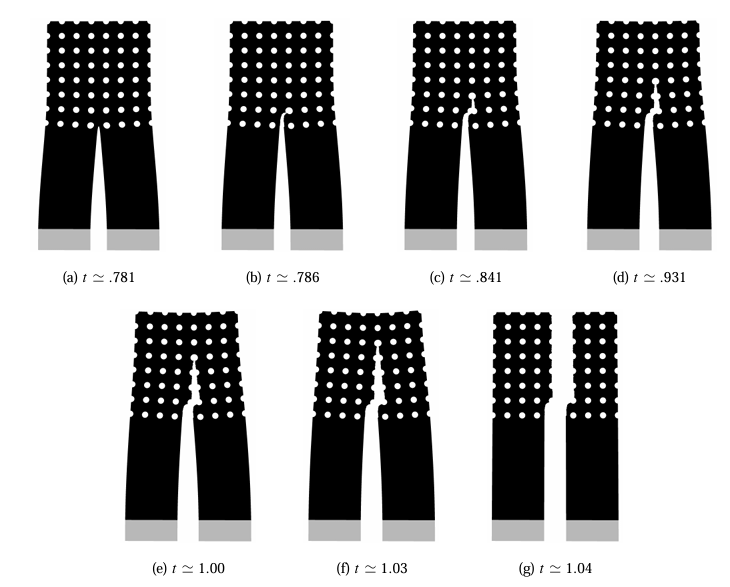
\includegraphics[width=0.8\textwidth]{FIG/BrittleFracture.png}
\caption{Crack propagation in brittle material, image taken from paper by Blaise Bourdin} % nb: cite?
\end{figure}
\end{frame}

% phase-field fracture model
\begin{frame}{Phasefield fracture model}

\begin{equation*}
	E_\ell(u,\alpha) = \int \frac{1}{2} (1 - \alpha)^2 A e(u) \cdot e(u) dx + \frac{G_c}{4 c_w} \int \frac{w(\alpha)}{\ell} + \ell \abs{\nabla \alpha}^2 dx
\end{equation*}
\begin{itemize}
\item $u$ is a vector field which defines the displacement
\item $\alpha$ is a scalar field that is 0 away from the crack and 1 on the crack
\item $e(u)$ is the strain tensor, $A$ the stiffness tensor
\item $\ell$ determines the accuracy of the approximation of the Hausdorff measure of the crack
\item $w(0)=0$, $w(1)=1$, $w'(x) \geq 0$, $w \in C^1(0,1)$, $c_w = \int_0^1 \sqrt{w(s)} ds$
\item $G_c$ is the critical energy release rate
\item The model is quasi-static: energy is minimized for a given time step/external work, then the model steps forward in time
\end{itemize}
\end{frame}

\begin{frame}{Alternate minimization}

Cracks propagate to minimize $E_\ell(u,\alpha)$.
To model this, we then need to minimize over both $u$ and $\alpha$:
\begin{equation*}
	\begin{bmatrix} F(u,v) \\ G(u,v) \end{bmatrix} = \begin{bmatrix} \dx{}{u} E_\ell(u,\alpha) \\ \dx{}{\alpha} E_\ell(u,\alpha) \end{bmatrix} = \begin{bmatrix} 0 \\ 0 \end{bmatrix}.
\end{equation*}

The energy $E_\ell$ is not convex in both variables, but it is convex if either $u$ or $\alpha$ is kept constant.
This leads to alternate minimization.
\begin{algorithm}[H]
	\caption{Alternate Minimization (AltMin)}
	\begin{algorithmic}[1]
		\State Make initial guess $\alpha_0$ and set $n=0$
		\While{$\norm{\alpha_{n+1} - \alpha_n}$ is greater than tolerance}
			\State Find $u_{n+1} = \argmin_u E_\ell(u, \alpha_n)$
			\State Find $\alpha_{n+1} = \argmin_\alpha E_\ell(u_{n+1},\alpha)$
		\EndWhile
	\end{algorithmic}
\end{algorithm}
\href{PLOT_GD_AltMinAnimation.mp4}{\textcolor{blue}{(animation)}}
\end{frame}

% MSPIN
\begin{frame}{Applying Newton (Kopanicakova, Kothari \& Krause, 2023)}

AltMin can be thought of as a fixed point iteration over $\alpha$:
\begin{equation*}
	\alpha_{n+1} = \text{AltMin}(\alpha_n),
\end{equation*}
which stops when $\alpha_{n+1}$ is sufficiently close to $\alpha_n$.

To accelerate the otherwise linear convergence, we can apply Newton's method to AltMin($\alpha$) - $\alpha$ after the minimization steps:
\begin{equation*}
	\begin{bmatrix} J_{uu} \\ J_{\alpha u} & J_{\alpha \alpha} \end{bmatrix}^{-1} \begin{bmatrix} J_{uu} & J_{u \alpha} \\ J_{\alpha u} & J_{\alpha \alpha} \end{bmatrix} \begin{bmatrix} u_* - u_n \\ \alpha_* - \alpha_n \end{bmatrix} = \begin{bmatrix} u_{n+1} - u_n \\ \alpha_{n+1} - \alpha_n \end{bmatrix},
\end{equation*}
where $J_{ij}$ is the second derivative of $E_\ell(u,\alpha)$ with respect to $i$ then $j$.

In practice, we solve this system inexactly and usually with some kind of backtracking to globalize Newton's method.
The resulting method is called multiplicative Schwarz preconditioning inexact Newton's method (MSPIN).
\end{frame}

\begin{frame}{Globalization techniques}

Newton's method needs globalization techniques to converge when the starting guess is far from a minimum.
The default choice is cubic backtracking:
\begin{algorithm}[H]
\caption{Cubic backtracking}
\begin{algorithmic}[1]
\State Inputs: current iterate $x_c$, search direction $p$, objective function $F(x)$
\State Set $\lambda_0 = 1$
\State Set $\lambda_1$ such that $x_p = x_c + \lambda_1 p$ minimizes the quadratic polynomial interpolating $F(x_c)$, $F(x_c + p)$ and $\nabla F(x_c)^\top p$
\While{$F(x_c + \lambda_1 p) \geq F(x_c)$ and $\norm{p} <$ some tolerance}
	\State Set $\lambda_2$ such that $x_c + \lambda_2 p$ minimizes the cubic polynomial interpolating $F(x_c)$, $F(x_c + \lambda_0 p)$, $F(x_c + \lambda_1 p)$ and $\nabla F(x_c)^\top p$
	\State $\lambda_0 \gets \lambda_1$, $\lambda_1 \gets \lambda_2$
\EndWhile
\end{algorithmic}
\end{algorithm}
\end{frame}

% parallelogram
\begin{frame}
\frametitle{Parallelogram minimization}

MSPIN is well-suited for a new kind of globalization technique because it requires finding two solutions for the same problem:
\begin{itemize}
\item the result from multiplicative Schwarz/AltMin, $x_c + q$, and;
\item the result from the Newton's method step, $x_c + p$.
\end{itemize}
This gives us two directions to look in, meaning we should seek our minimum in a parallelogram.

\centering
\begin{tikzpicture}
	\node[below left] at (0,0) {$x_c$};
	\node[below right] at (3,0) {$x_c + p$};
	\node[above left] at (1,2) {$x_c + q$};
	\node[above right] at (4,2) {$x_c + p + q$};
	\draw (0,0) -- (3,0) -- (4,2) -- (1,2) -- cycle;
\end{tikzpicture}

\end{frame}

\begin{frame}
\frametitle{Parallelogram minimization}

Given an objective function $F(x)$, minimize the polynomial $P(i,j) = ai^2 + b ij + cj^2 + d i + e j + f$, where
\begin{align*}
	f = & F(x_c),
	& e = & \nabla F(x_c)^\top p,
	& d = & \nabla F(x_c)^\top q,
	\\ c = & F(x_c + p) - e - f,
	& a = & F(x_c + q) - c - f,
\end{align*}
\begin{equation*}
	b = F(x_c + p + q) - F(x_c + p) - F(x_c + q) + f,
\end{equation*}
in the region where $0 < i, j < 1$.
\begin{equation*}
	\begin{bmatrix} i_{\text{min}} \\ j_{\text{min}} \end{bmatrix} \in \set{ \begin{bmatrix} \frac{-2cd + be}{4ac - b^2} \\ \frac{-2ae + bd}{4ac - b^2} \end{bmatrix}, 
	\begin{bmatrix} 0 \\ -\frac{e}{2c} \end{bmatrix}, \begin{bmatrix} -\frac{d}{2a} \\ 0 \end{bmatrix}, \begin{bmatrix} 1 \\ -\frac{e + b}{2c} \end{bmatrix}, \begin{bmatrix} -\frac{d + b}{2a} \\ 1 \end{bmatrix}, 
	\begin{bmatrix} 0 \\ 1 \end{bmatrix}, \begin{bmatrix} 1 \\ 0 \end{bmatrix}, \begin{bmatrix} 1 \\ 1 \end{bmatrix} }
\end{equation*}
Our new minimum is $x_n = x_c + i_{\text{min}} q + j_{\text{min}} p$.
\end{frame}

\begin{frame}
\frametitle{Example calculations}

\begin{figure}
	
\includegraphics[height=18em]{FIG/EX_CTFM_AltMin01.png}
	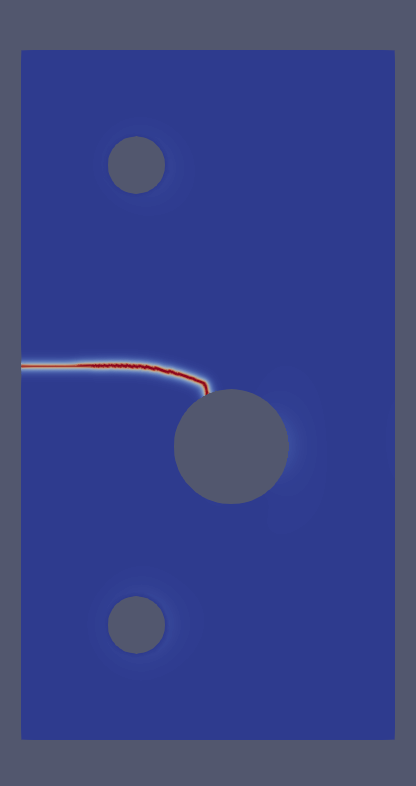
\includegraphics[height=18em]{FIG/EX_CTFM_AltMin02.png}
	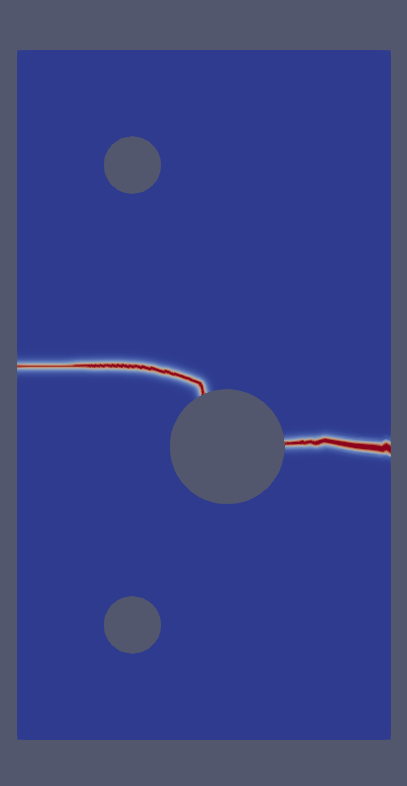
\includegraphics[height=18em]{FIG/EX_CTFM_AltMin03.png}
\end{figure}

\end{frame}

\begin{frame}
\frametitle{Computation time}

\begin{figure}
	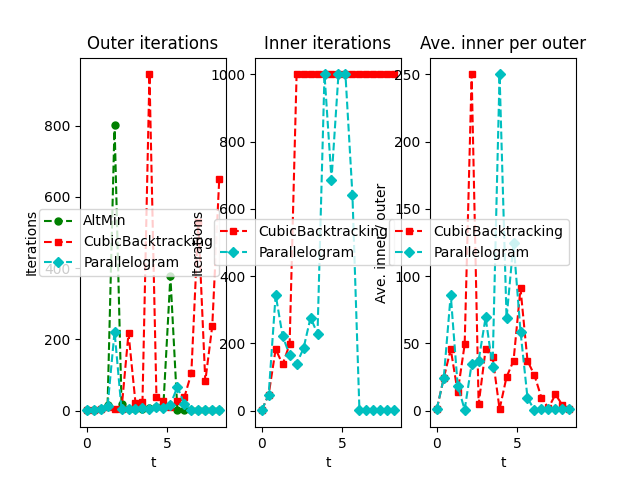
\includegraphics[width=\textwidth]{FIG/FIG_CTFM_its.png}
\end{figure}

\end{frame}

\begin{frame}
\frametitle{Summary}

Domain decomposition and Schwarz methods permit parallelization and can improve problem conditioning.
We need additional methods to accelerate convergence rates above linear.

Newton-Schwarz methods need globalization techniques to stabilize them for difficult problems.
Parallelogram minimization combines both the Newton and Schwarz directions for faster convergence.

\end{frame}

\begin{frame}

\begin{center}
\LARGE{Thank you}
\end{center}

\end{frame}

\begin{frame}
\frametitle{References}
\fontsize{10pt}{0}{
\begin{itemize}
\item Bourdin, B. \textbf{Numerical implementation of the variational formulation for quasi-static brittle fracture.} \textit{Interfaces and Free Boundaries} 9 (2007).
\item Kopanicakova, A., Kothari, H. \& Krause, R. \textbf{Nonlinear field-split preconditioners for solving monolithic phase-field models of brittle fracture.} \textit{Computer methods in applied mechanics and engineering} 403 (2023).
\item Cai, X.C. \& Keyes, D.E. \textbf{Nonlinearly preconditioned inexact Newton algorithms.} \textit{SIAM Journal on Scientific Computing} 24 (2002).
\end{itemize}
}
\end{frame}

\end{document}